\section{Dedicated Detectors for LLPs}
\subsection{Introduction}

Some boilerplate about how, in cases of ultra-low-mass particles, ultra-long lifetimes, or unusual LLP charged, it is hard to trigger on and/or reconstruct the events in the main ATLAS, CMS, and LHCb detectors. This has led to new proposals and experiments to look for LLPs in new regimes that are otherwise inaccessible at the LHC. These experiments provide the best sensitivity to new millicharged LLPs, magnetic monopoles, and other models such as Higgs-portal hidden sectors, dark photons, and Majorana neutrinos.


\subsection{A Compact Detector for Exotics at LHCb (CODEX-b)}
\label{sec:CODEX-b}

As discussed elsewhere in the white paper, LLPs are theoretically well motivated and come in wide range of masses and lifetimes. ATLAS and CMS have excellent sensitivity for fairly high mass LLP's, regardless of their lifetime  (see e.g.~\cite{CMS:2016ybj,Aaboud:2016dgf,CMS-PAS-EXO-16-003,ATLAS-CONF-2016-103}). Low mass and/or softer final states are more challenging due to both background and triggering limitations. In the short lifetime regime, for $c\tau$ of the scale of the VELO, LHCb has sensitivity to somewhat lower masses and can trigger on softer muonic final states, generating complementary reach provided the LLP has a significant branching ratio to muons~\cite{Aaij:2017mic,Aaij:2016xmb,Aaij:2016isa,Aaij:2015ica,Aaij:2014nma}. Finally the low mass/soft final states with rather long lifetimes are challenging for all three experiments. These signatures can be covered partially by NA62~\cite{NA62:2017rwk} operating in beam dump mode, or by SHiP~\cite{Alekhin:2015byh}, or by dedicated LHC experiments like MATHUSLA~\cite{Chou:2016lxi}, FASER~\cite{Feng:2017uoz} or CODEX-b \cite{Gligorov:2017nwh}. Of these options, only MATHUSLA and CODEX-b could gather a large sample Higgs bosons.



The CODEX-b proposal involves housing a (sub)detector in the LHCb cavern in a space approximately $25$\,m from the interaction point (IP8), behind the 3m thick concrete UXA shield wall. This space is presently occupied by the LHCb data acquisition, but will become available pre-Run 3 once it is relocated to the surface. The layout of the cavern is shown in Fig.~\ref{fig:LHCbCav}, with the location of CODEX-b overlaid. 
%In particular the LHCb data acquisition system is currently housed behind the 3m thick concrete UXA shield, but will be moved to the surface during the pre-run 3 upgrade. 
The nominal CODEX-b configuration features a $10$$\times10$$\times10$\,m volume instrumented with RPC tracking layers or other off-the-shelf tracking technology, as well as roughly $25$ interaction lengths of shielding near IP8 -- e.g. $4.5$\,m of Pb --  to suppress primary and secondary $K_L$, neutron and other hadronic backgrounds. This shield requires an active muon veto with an efficiency of $\mathcal{O}(10^{-5})$, in order to reject muon or other charged particle induced backgrounds in the downstream parts of the shield: The veto is located several metres within the shield such that neutral particle induced backgrounds remain suppressed. We refer to Ref.~\cite{Gligorov:2017nwh} for a study of a proof-of-concept  example detector layout and corresponding tracking efficiency, as well as a detailed study of the backgrounds.
% It should be emphasized that for the purpose of demonstrating reach, tracking efficiencies and background control, Ref.~\cite{Gligorov:2017nwh} studied a particular proof-of-concept implementation for CODEX-b. 
More ambitious technologies, including calorimetry, precision time-of-flight, or integration into the LHCb readout may also be feasible.

\begin{figure}[t]\centering
	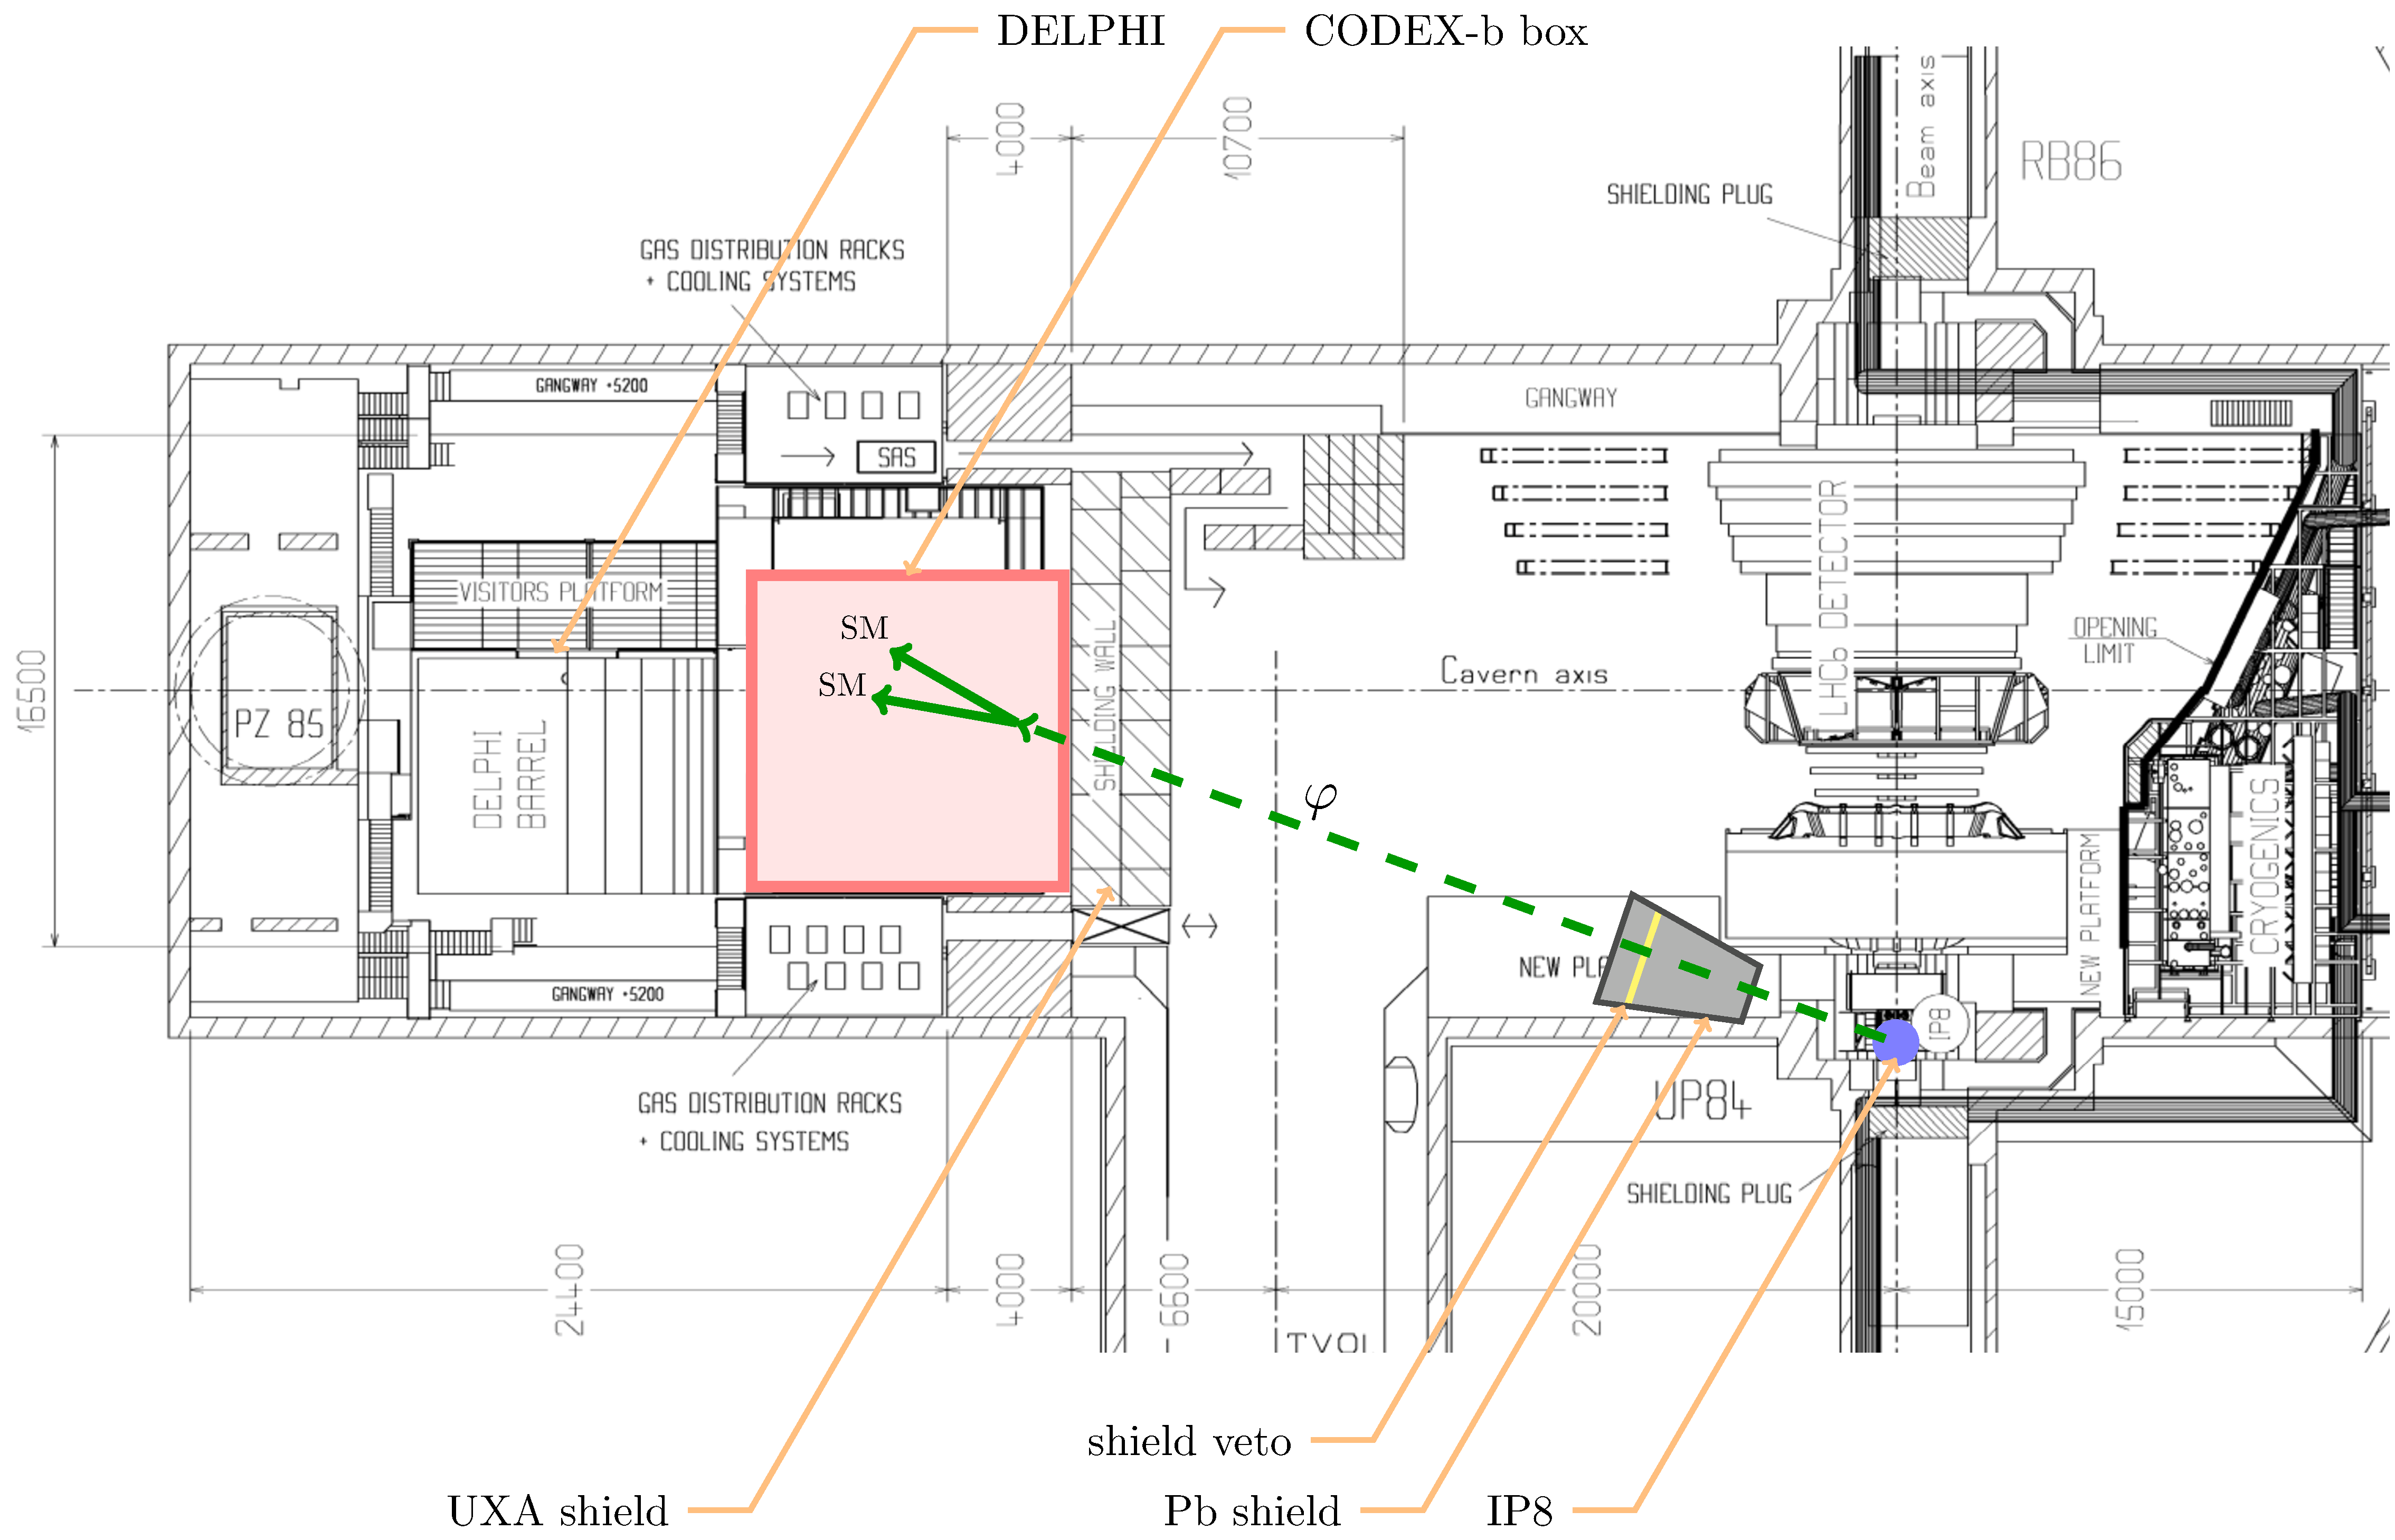
\includegraphics[width = 0.75\linewidth]{plots/LHCbCavern}
	\caption{Layout of the LHCb experimental cavern UX85 at point 8 of the LHC~\cite{cavern}, overlaid with the proposed CODEX-b location.} 
	\label{fig:LHCbCav}
\end{figure}

For the purposes of this white paper, we quantify the reach of CODEX-b for two benchmark models:
% (i) A light scalar which mixes with the Higgs and a (ii) a dark photon which is primarily produced through an exotic Higgs decay.
First we consider light scalar field, $\X$, that mixes with the SM Higgs boson. If $m_\X\lesssim$ 5 GeV, the production mode is primarily through 
inclusive $b \rightarrow s \X$ decays~\cite{Willey:1982dk,Chivukula:1988lo,Grinstein:1988yu}. The LLP $\X$ subsequently decays back to SM fermions through the same Higgs portal. The reach in terms of $m_\X$ and the mixing angle $s_\theta$ is shown in the left-hand panel of Fig.~\ref{fig:ThVM}. CODEX-b significantly extends the projected reach of LHCb using only VELO-based displaced vertex reconstruction, and covers part of the projected parameter of SHiP~\cite{Lanfranchi:2243034} and MATHUSLA  \cite{Evans:2017lvd}. Studies of the potential LHCb reach to longer lifetimes using downstream tracking are ongoing~\cite{Sierra:2017tw,Aaij:2244312}. The right-hand panel of Fig.~\ref{fig:ThVM} indicates the reach for more general models, where the lifetime and production rate of $\X$ are unrelated.


\begin{figure}[t]\centering
	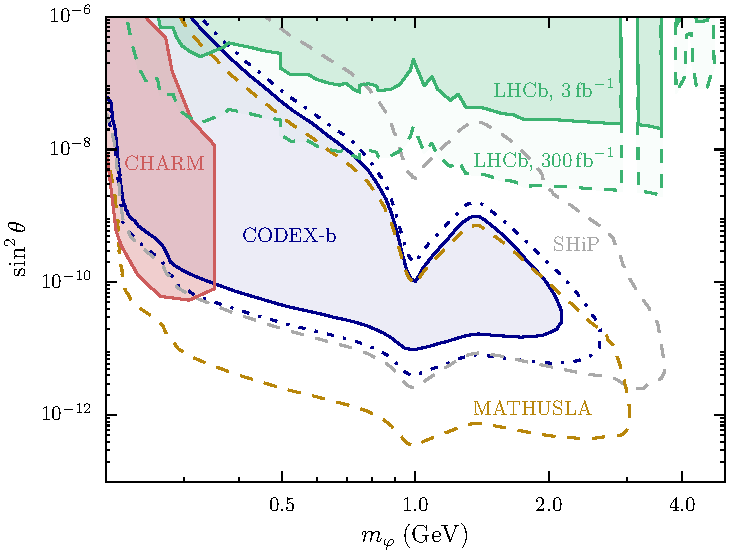
\includegraphics[height =  5cm]{plots/moneyplot_whitepaper.pdf}\hspace{2cm}
	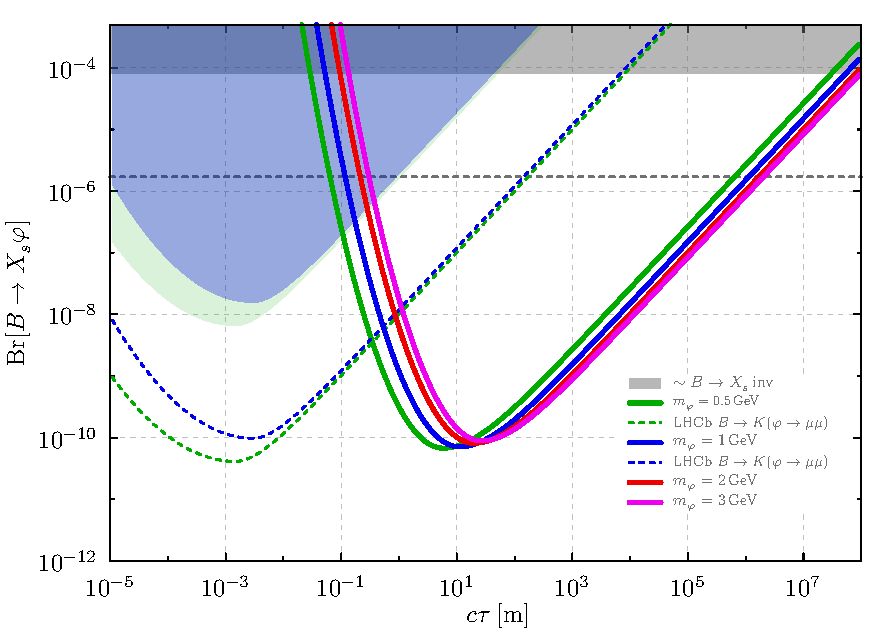
\includegraphics[height = 5cm]{plots/cTauB}
	\caption{\emph{Left:} CODEX-b reach for $B\rightarrow X_s\X$ in the $s^2_\theta$--$m_\X$ plane. Solid (dot-dashed) line assumes $\mathcal{L} = 300\, \text{fb}^{-1}$ ($\mathcal{L} = 1\, \text{ab}^{-1}$).
	\emph{Right:} Inclusive CODEX-b $B \to X_s \X$ reach (solid lines). The shaded regions (dashed lines) indicate current LHCb limits (300$\,$fb$^{-1}$ projection) from $B \to K(\X \to \mu\mu)$, rescaled to the inclusive process and assuming $\text{Br}[\X \to \mu\mu] \simeq 30\%$  and $10\%$ for $m_\X = 0.5$~GeV and $1$\,GeV, respectively. Gray shading and dashed line indicate respectively the approximate current~\cite{PDG:2016} and Belle II projected~\cite{BelleIIreport} limits from $B \to K^{(*)}\nu\bar\nu$ precision measurements.	
	} 
	\label{fig:ThVM}
\end{figure}

For our second benchmark, we consider a dark boson, $\gd$, produced through the exotic Higgs decay $h\rightarrow\gd\gd$. For concreteness we take $\gd$ to be a spin one field which can decay through mixing with the Standard Model photon~\cite{Schabinger:2005ei,Gopalakrishna:2008dv,Curtin:2014cca,Strassler:2008bv}.  In this benchmark, the production and decay are therefore controlled by different portals. The projected reach is shown in Fig.~\ref{fig:HXX}, overlaid with the reach of ATLAS \cite{Coccaro:2016lnz,ATLAS-CONF-2016-042} and MATHUSLA \cite{Chou:2016lxi}. In particular at low $\gamma_d$ masses, CODEX-b complements and significantly extends the reach of ATLAS and CMS.




\begin{figure}[t]\centering
	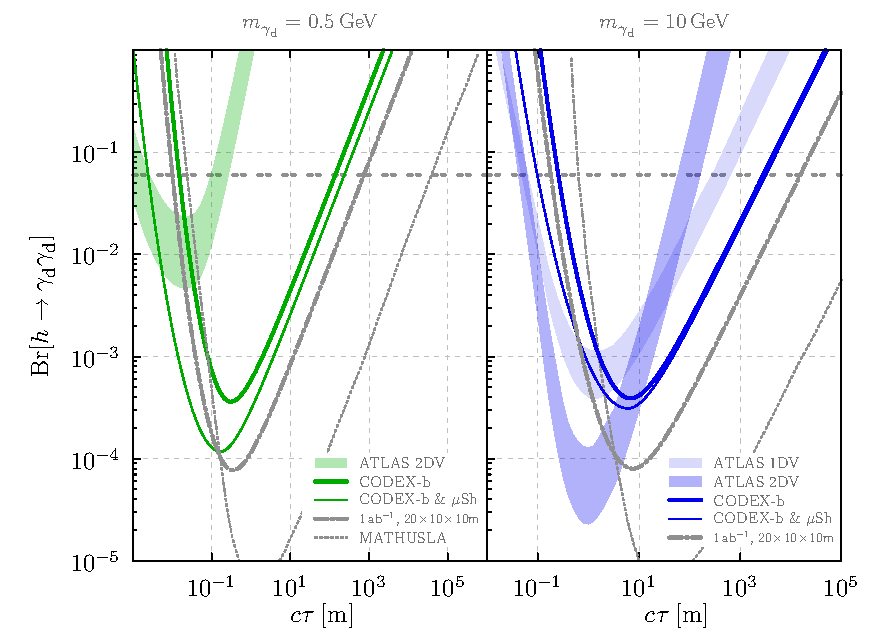
\includegraphics[height =  6cm]{plots/cTau_panel}
	\caption{Higgs decay to dark photon reach with and without the muon shadow (`$\mu$Sh'). The $\gd \to \mu\mu$ branching ratio is taken from $e^+e^-$ data~\cite{Meade:2009rb}. Also included is the optimistic CODEX-b reach with $\mathcal{L} = 1$\,ab$^{-1}$ and a larger volume, assuming DELPHI is removed. }
	\label{fig:HXX}
\end{figure}
